\documentclass[12pt,a4paper,oneside,titlepage]{article}

\usepackage{hyperref}
\usepackage{graphicx}
\usepackage{pgfgantt}
\usepackage{lscape}
\usepackage[a4paper]{geometry}

\begin{document}
\title{GC02 Team 7 Project Report \\ MINAP Mobile Application}
\author{Amer Kamil Zainal Abidin, Ke Wei, Marco Corrales Estrada}
\maketitle

\tableofcontents
\newpage
\section{Background}
\subsection{MINAP/NICOR}
The Myocardial Ischaemia National Audit Project (MINAP) investigates the management of heart attacks. Participating hospitals and ambulance services are provided with a record of their quality of management. These records are then compared to national and international clinical standards. The National Institute of Cardiovascular Outcomes Research (NICOR) is a partnership of clinicians, IT experts, analysts, academics and managers. Its mission is to "provide information to improve heart disease patients' quality of care and outcomes". Using different audits, MINAP being one of them, NICOR aims to provide the NHS, government and regulatory bodies real world data to be used in patient care \footnote{\href{http://www.ucl.ac.uk/nicor/audits/minap/publicreports}{MINAP Reports}}\footnote{\href{http://www.ucl.ac.uk/nicor}{NICOR Website}}. 

\subsection{Web Application}
Participating hospitals are requested to enter all patients with suspected heart attack into MINAP's central database system. Data are collected by nurses and other clinical audit staff and entered in a dedicated web application. This web application collects all patient data, from demographics to diagnosis and release information. As it stands, the web application contains a 130 field dataset that is updated every two years (latest revision, June 2013); it is currently only available to the web browser Internet Explorer versions 9 or below. The data is then validated against a set of rules which include, but are not limited to, value range checks, date range checks, data type checks and encryption rules. Once completed, records are stored on MINAP's Domino server\footnote{IBM Domino is used for enterprise collaboration, and is used primarily for its Lotus Notes capabilities in this instance}.

\subsection{Client}
The project's primary point of contact is Lucia Gavalova, Project Manager for the MINAP project, who we will refer to as the 'client' throughout this document (unless stated otherwise). Sue Manuel, MINAP's web app developer has also been a key stakeholder throughout the course of this project.

\newpage
\section{Requirements}
\textit{The following requirements have been formulated from a series of client meetings and e-mail communication, available in brief under Client Communication.}

\subsection{Overview}
Patient data record creation is currently restricted to when the nurses and other clinical audit staff are sitting in front of a computer. This would often be quite some time after a patient has been identified as being eligible for being entered into the MINAP dataset. A reduced-function mobile solution of the current web app was proposed by our client as a means of starting a patient record in MINAP's data set, allowing for prospective data collection. Completion of the record is expected to be done later on using the web app (using a full sized keyboard and screen).

\subsection{Use Cases}
The system's use case we are concerned with for our app can be modelled by the following table. Although the user-facing view of the system is fairly simple, most of the application logic lies in the interdependency and validation checks of the values entered by the user. 

\begin{center}
\begin{tabular}{|l|}
	\hline
	A nurse or clinical audit staff wants to create a record\\ \hline
	She first needs to login to the server with her credentials\\ \hline
	She then selects an option to create a new record\\ \hline
	She then is brought to a page to enter in her initial diagnosis\\ \hline
	If she doesn't understand a field, she can click on a button for help\\ \hline
	She then enters the patient details into a data input field\\ \hline
	If the data entered is invalid, a pop-up will appear, \\prompting her for correction\\ \hline
	She can then navigate through each page using 'next' buttons, \\or through a navigation map\\ \hline
	Throughout this process, she will save the data to the server by \\clicking a save button\\ \hline
	Once complete, she logs out of the system\\ \hline
	\end{tabular}
\end{center}
\subsection{Functional Requirements}
\subsubsection{User Authentication and Security}
As with the web application, the user must login to the central server prior to using the mobile app for data input. For security purposes, the user authentication details should not be held on the device beyond the initial authentication phase (or instead, use tokens), and all sensitive data retrieved from the server and created on the device should be destroyed at the end of a user session.
\subsubsection{Data Collection}
In order to create a patient record, the app needs to provide the user with forms for data entry. Depending on the data fields, certain format restrictions are imposed, for example: date and time related fields are in the dd/mm/yy hh:mm format; combo boxes; and numeric only data fields. Data fields should be divided into sections (pages) based on the current web app structure for familiarity. Data entered in by the user should be stored locally for the duration of the session, and ideally sent to a server once validated\footnote{See Data Submission}.
\subsubsection{Data Validation}
Validation currently occurs on the web app automatically at the point of exiting a data input object, page, or on saving. All 130 fields within the dataset must pass at least one validation rule. Certain fields will then either trigger additional validation rules involving other fields, default values to other fields, and/or open new sections of data collection to be filled out. Our app should follow this behaviour (with a subset of data) to ensure data integrity.
\subsubsection{Data Submission}
Once all mandatory data is entered and all validations rules have been passed, the user will be able to store the local record to a SQLite database. Due to time constraints, the team was unable to test calls to a web service of our own design as agreed with the client (20/11/13 Meeting). However, the SQLite database should prove to be flexible if used in future implementations as it is self-contained and follows the dataset's specifications.
\subsubsection{Mobile Usability}
Since the app will be running on smart phones (our target platform), factors such as the screen size, touch navigation, and use of an on-screen keyboard have to be taken into account during the user interface design phase. Certain features in the current web app (e.g. navigation and data submission) are not intuitive and need to be rethought for mobile use, but should still retain the familiarity of the existing interface. 

\subsection{Architectural Requirements}
The core purpose of our mobile application is to provide proof of concept for a solution what would offer a starting point for record creation. To that end, we came to a mutual agreement with the client that the original dataset be reduced from 130 fields. In exchange for reducing the volume of data, certain architectural requirements were requested so as to create a framework for future work to build upon (e.g. porting the application to other platforms).
\subsubsection{Web Services}
Although we have reached an agreement that we will not actually need to touch the live Domino Server, there are certain functions that our application will have to implement to ensure future compatibility with MINAP's technology stack (IBM Lotus Notes on Domino Server 8.5.3). Processes such as how data will be retrieved from the server and authentication processes should be modelled into the system as stubs that can be easily implemented at a later stage in the development of the app. Further research into the topic of communication with the server from other services was also deemed useful, since the client was unable to give a clear answer as to how this could be done.

\newpage
\section{Target Mobile Platform}
THIS SECTION IS TO BE REWRITTEN
\\ \\
Our client has been unsure about the preferred target platform of the audience of our mobile app. To help better inform this decision, we have designed a user device survey which the client has agreed to running over the period of a few months, with a suggested completion date within 3 weeks of rolling out. The primary purpose of pushing out this survey is to better inform decisions of what secondary platforms should be supported to increase mobile app uptake by hospital staff. Despite this, due to the short time-frame imposed on us by GC01, we have mutually agreed to target Android mobile phones as the primary platform. More details regarding the device survey can be found in the Appendix.
\\ \\
THIS SECTION IS TO BE REWRITTEN

\newpage
\section{User Interface}
As part of ensuring our understanding of the requirements were in line with the client's expectations, we sketched out a preliminary user interface (UI) and presented our ideas to our client. The order in which each page was presented is indicated by red arrows. A summary of the key points relating to UI during our conversation are included below.

\subsection{Initial User Interface Feedback}
Client response:
\begin{itemize}
	\item happy with proposal of similar design to web app
	\item current (web app) record search criteria is non-specifiable (simple text match); this behaviour is sufficient for the mobile app
	\item request for an application tutorial for "non-techie" users
	\item navigation menu: a simplified version of the map could be used for mobile
	\item an 'auto-save' feature would be useful ("like Microsoft Word") in case of battery loss, device breakage, or more pressing matters to attend to (i.e. emergency)
\end{itemize}
\subsubsection{Commentary and Response}
We have accepted the feedback from the client as being in line with our initial requirements. However, the request for an auto-save feature in the app would violate the privacy requirements of having volatile local data. A way to mitigate this would be to save the record to a 'draft' database when auto-saving (i.e. "submitting" a record without performing validation-on-send), but is a low-priority feature at this point.
\subsubsection{UI Tweaking}
After taking these comments on board, we have more formally modelled the user's flow of use through the app, mapping each UI element to Java's graphical implementation classes. It is worth noting that the UI is still in its initial stages, pending further adaptation for mobile use.

\newpage
\section{Software Design}
\subsection{Class Diagrams}
\subsection{Data Dictionary}




\newpage
\section{Project Management}


\subsubsection{Work Packages}



\begin{landscape}
\subsubsection{Gantt Chart}
\begin{ganttchart}[
	hgrid,
	vgrid,
	time slot format=isodate
	]{2013-11-01}{2013-11-30}
	\gantttitlecalendar{year, month=name, day} \\
	\ganttgroup{Requirements Gathering}{2013-11-01}{2013-11-15} \\
	\ganttmilestone{GC01 Milestone 1}{2013-11-24} \ganttnewline
	\ganttgroup{InitialDevelopment}{2013-11-16}{2013-11-30} \\
\end{ganttchart}


\begin{ganttchart}[
	hgrid,
	vgrid,
	time slot format=isodate
	]{2013-12-01}{2013-12-31}
	\gantttitlecalendar{year, month=name, day} \\
\end{ganttchart}


\begin{ganttchart}[
	hgrid,
	vgrid,
	time slot format=isodate
	]{2014-01-01}{2014-01-25}
	\gantttitlecalendar{year, month=name, day} \\
\end{ganttchart}

\end{landscape}

\newpage
\section{Teamwork}
\subsection{Team Roles}
Team roles were assigned based on the recommended list provided in the GC01 document requirements.
\begin{center}
    \begin{tabular}{ | l | l | p{5.4cm} |}
    \hline
    Name & Primary Role & Secondary Role \\ \hline
    Marco \textbf{David} Corrales & Secondary Team Lead & Primary Developer \\&& Background Researcher \\&& UI Designer \\ \hline
     Amer \textbf{Kamil} Zainal & Primary Team Lead & Technology Researcher \\&& Software Tester \\&& Systems Designer \& Analyst \\&& Documentation Lead \\ \hline
     \textbf{Ke} Wei & Client Main Contact & Secondary Developer \\&& Data Designer \\&& Device \& Deployment Tester \\ \hline
    \end{tabular}
\end{center}

\subsection{Teamwork Commentary}
\subsubsection{Team Workflow}
\href{https://trello.com}{Trello}\footnote{Information disclosed on Trello are private to the team} has been used extensively by the team for information organisation. Agendas for the next meeting are decided at the end of each meeting, with unfinished items of the day deferred; ensuring that each agenda is a summary of what was achieved at each meeting. To supplement this, any details (e.g. comments, photos, resources) related to the meeting are included in a separate section with a corresponding date. 

To further consolidate our memory of team progress, our primary developer has been updating a \href{http://akz08.github.io/minap-mobile/}{blog} (http://akz08.github.io/minap-mobile/) summarising our meeting outcomes. Due to the public nature of blogs, we have ensured to omit any client identifying information to avoid any potential privacy problems. The blog should however be understandable upon reading the entirety of this report.

For code sharing, we currently use a private \href{https://github.com}{GitHub} repository which is worked on by all members of the team. GitHub's repository wiki functionality is used for collaboration of more long-form documentation (e.g. writing this report) and structured ordering of resources.

To avoid having to check both services frequently, we also use \href{https://www.flowdock.com/}{FlowDock} to easily track changes on both GitHub and Trello.
\subsubsection{Task Assignment}
Team members typically select the work packages outlined at the end of each meeting, but assignment of tasks tend to gravitate towards the team roles previously tabulated. 
\subsubsection{Meetings}
The team typically meets every workday to complete work together. Some team members pick up work to be done on their own time to help meeting productivity.

\newpage
\appendix
\newgeometry{left=1cm}
\section{Data Dictionary}
\subsection{Patient Class}

\begin{center}
	\begin{tabular}{| l | p{5cm} |}
	\hline
	\textbf{AdminStatus} & \textbf{$<<$extends Value$>>$} \\ \hline
	\textasciitilde com.ucl.appteam7.minapmobile.model.values.DemographicsAdmission	 & \\ \hline
	$<<$import$>>$ com.ucl.appteam7.minapmobile.model.Value& \\ \hline \hline
	- \underline{adminStatus} : Byte & Holds the short code for patient's admission status \\ \hline
	& \\ \hline
	& \\ \hline	
	\end{tabular}
\end{center}
\restoregeometry

\newpage
\section{Client Communication}
Our first contact with the client was on Monday 28th October, with a short meeting outlining the aims of the MINAP project the following day. We have had 3 meetings with the client and other members of MINAP/NICOR so far. All meetings have been recorded (audio) with the consent of those present. A brief summary of the people present and key talking points are outlined below.
\subsection{Project Introduction \& Requirements (1/11/13)}
\subsubsection{Meeting Agenda}
To get a clear understanding of the project requirements, and to hammer down a realistic project specification that can be delivered within 3 months. 
\subsubsection{People Present}
App Team 7, Lucia Gavalova (Project Manager), Fabian D'Souza (Server Admin), Owen Nicholas, "Tech-guy"
\subsubsection{Discussion}
\begin{enumerate}
	\item Feasibility of creating a mobile app from the current web app 
	\begin{enumerate}
	\item Tech-guy suggests that it is likely that XPages (open-source javascript framework used for business solutions) is the only way of creating an app 
	\item Tech-guy has no idea if the Domino server housing the MINAP data can be accessed via mobile, though suggests XPages as a starting point 
	\end{enumerate}
	\item Fabian called in to hopefully get better ideas on how to implement a mobile solution working with the current technology stack 
	\begin{enumerate}
	\item Recommends looking at using IBM Lotus Notes (client software to Domino server) as an intermediary for the app 
	\item Suggests that Java could theoretically be used by including a notes.jar file which allows the development of a Lotus Notes plug-in 
	\item Promises to send relevant links that may help with finding a solution 
	\end{enumerate}
	\item Owen and tech-guy suggests that the validation of 130 values of the MINAP dataset will definitely take more than 3 months.
\end{enumerate}
\subsubsection{Outcomes}
We were thoroughly confused after the meeting with regards to the Domino Server. Fabian did send the e-mail but it only served to confuse even further. We however decided to spend some time researching on the possible ways to communicate with this legacy technology. Lucia provided us with documents containing the full set of data values and validations rules for us to understand. We also provided details to gain access to MINAP’s development server to have access to the current web application - this was only processed 2 weeks later.

\subsection{UI Feedback (15/11/13)}
\subsubsection{Meeting Agenda}
To obtain client feedback on our preliminary UI, clarify confusions about the MINAP dataset, validation, and use. The target platform needed to be locked down.
\subsubsection{People Present}
App Team 7, Lucia Gavalova
\subsubsection{Discussion}
\begin{enumerate}
	\item Marco David Corrales presented the UI sketches to Lucia 
	\begin{enumerate}
	\item Lucia is happy with the proposal of a design similar to the current web app
	\item Mentions that the search functionality can just mirror the simple search in the current web app
	\item Requests that a tutorial for “non-techie” users 
	\item David notes down minor comments on UI sketches 
	\end{enumerate}
	\item Team requests a simplified version of the navigation map (and by extension, the 130 value dataset)
	\begin{enumerate}
	\item Lucia informs us of her initial motivation for a MINAP mobile app 
	\begin{enumerate}
		\item Mobile app serves as a starting point for medical staff to create a record for patients eligible to be monitored through MINAP when visiting non-cardiac wards 
		\item This helps alleviate the current problem of having positively skewed outcomes as the current patients being recorded are in specialist wards, and more likely to receive treatment when needed 
	\end{enumerate}
	\item The mobile app could therefore exist with just a subset of the functionality of the existing web app 
	\end{enumerate}
	\item Lucia requests an auto-save feature “like Microsoft Word” to allow sessions to be resumed later within the same day 
	\item Amer Kamil Zainal requests if a survey could be designed to get a solid feel of the target audience’s primary mobile operating system 
	\begin{enumerate}
	\item Lucia agrees - Kamil promises to design survey
	\end{enumerate}
\end{enumerate}
\subsubsection{Outcomes}
We managed to come to a mutual agreement that the mobile app could serve its main purpose by implementing only a subset of the total MINAP dataset. Lucia promised to send a document detailing the exact values that would need to be included to fulfil this requirement - the document was received some time after the next meeting. A flow diagram of the survey was completed and handed over to Lucia at the next meeting.

\subsection{Developer Session (20/11/13)}
\subsubsection{Meeting Agenda}
To understand how the current web app works and how it interacts with the Domino Server; to hand over the device survey flow chart for critique and deployment on SurveyMonkey.
\subsubsection{People Present}
App Team 7, Lucia Gavalova, Sue Manuel (Developer), Fabian D'Souza
\subsubsection{Discussion}
\begin{enumerate}
	\item Sue informs that the web app is made in Javascript, running on top of a Lotus Notes form (in turn, running on the Domino Server) 
	\item The Javascript methods use the Lotus Notes interface to retrieve data from the database 
	\item Sue mistakenly tells that validation of values is all server-side - a major setback if correct 
	\item Fabian called in to verify server-side validation claims - validation is client-side 
	\item Team request to have a copy of client-side validation code to cross-check with the data validation documents given 
	\item Discussion with Fabian regarding connecting to Domino Server
	\begin{enumerate}
	\item Team confirms research on how to communicate with Domino Server is correct
	\begin{enumerate}
		\item The Domino Server allows the creation of a web service (consumer and provider) 
		\item This would make the server be compatible with any application that can consume a web service 
	\end{enumerate}
	\item Fabian however insists that making our app communicate with a Domino Server is not a key priority, and that spinning off another web server (e.g. Apache + Microsoft SQL Server) with a similar web service capabilities will satisfy the requirements
	\end{enumerate}
	\item Device survey flow diagram presented and accepted as is by Lucia
\end{enumerate}
\subsubsection{Outcomes}
The team is now confident in delivering an application with the scaled-down specifications (fewer than 130 validations and Domino Server compatibility not being a priority). A link to the SurveyMonkey device survey was sent to the team, pending approval (by the team). However, due to the reduction of requirements occurring so close to the first report milestone (24/11/13), the team was unable to fully capture this more manageable system in Java.

\newpage
\subsection{Device Survey}
Draft proposal: To determine how many target medical personnel own smartphones (or considering purchase in the near future), and would use it in a work setting. + find out specific OS and screen sizes via requesting visit of a site on their mobile (loaded with Google Analytics). 
\begin{figure}[h!]
\centering
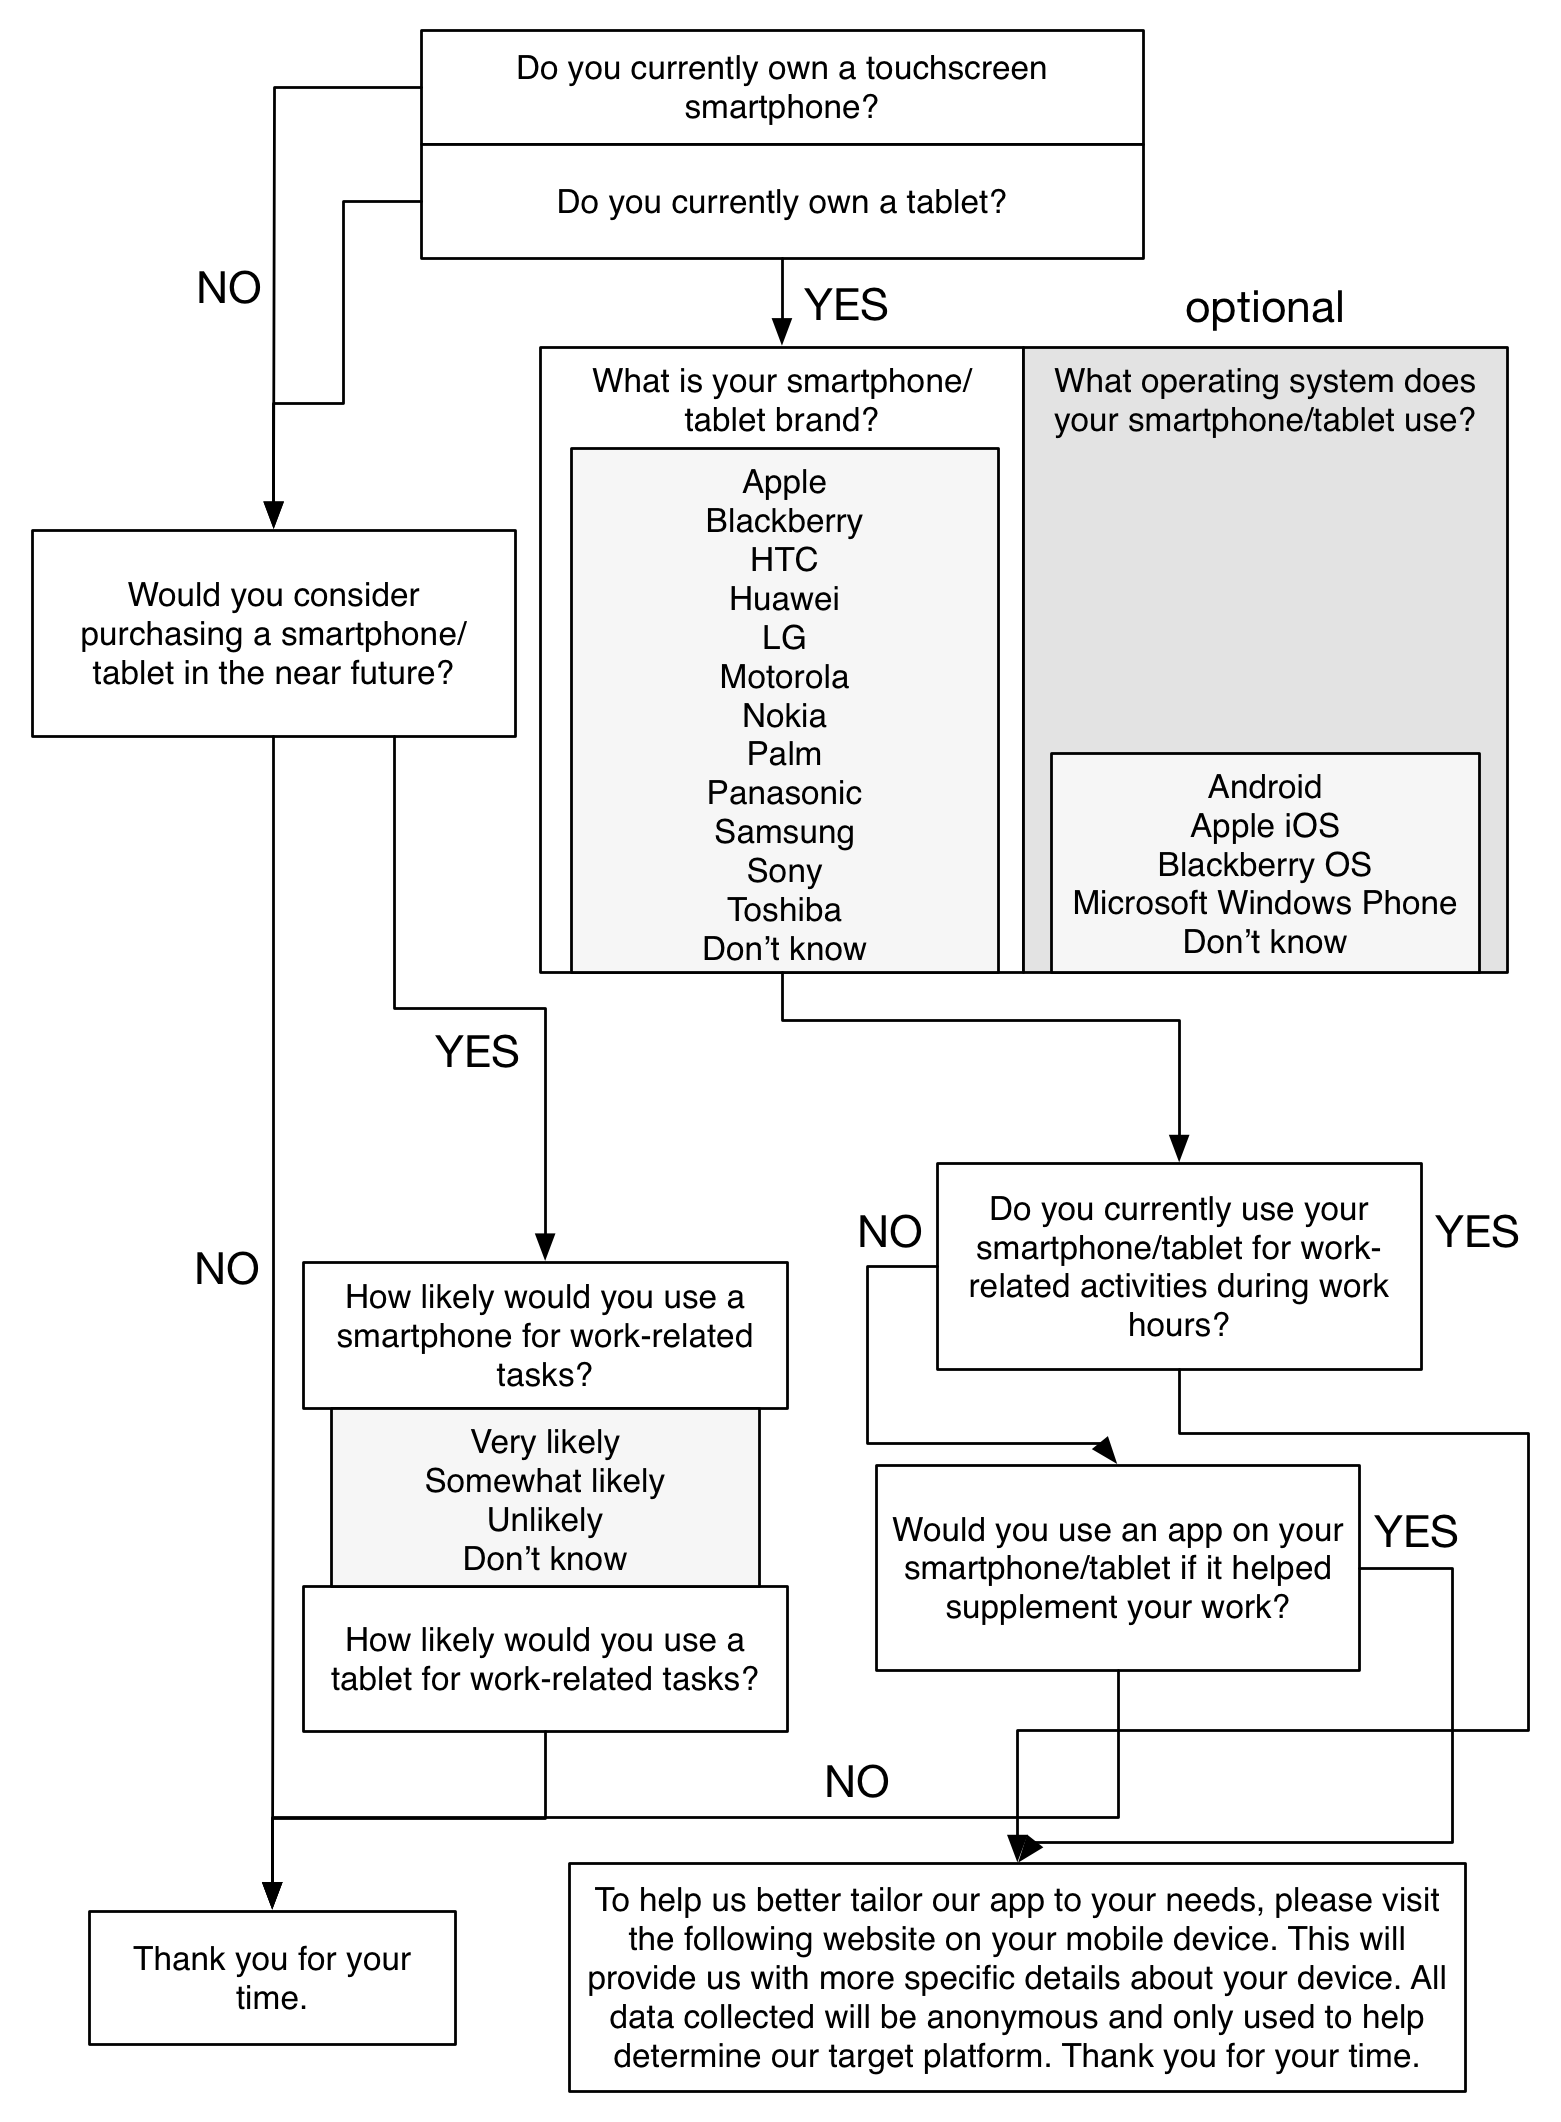
\includegraphics[scale=0.53]{img/device-survey.png}
\caption{Initial survey flow}
\end{figure}
\\
It was decided through client feedback that the survey flow logic could be replaced with a simple one-page linear survey due to the straightforward nature of the questions. The contents of the final survey are below.
\paragraph{Final SurveyMonkey Survey}
\begin{enumerate}
\item Do you currently own a touchscreen smartphone or a tablet?
\begin{enumerate}
\item Smartphone only
\item Tablet only
\item Smartphone and tablet
\item Neither
\end{enumerate}
\item Would you consider purchasing a smartphone/tablet in the near future?
\begin{enumerate}
\item Yes
\item No
\end{enumerate}
\item What is your smartphone/tablet brand?
\begin{enumerate}
\item Apple
\item Blackberry
\item HTC
\item Huawei
\item LG
\item Motorola
\item Nokia
\item Palm
\item Panasonic
\item Samsung
\item Sony
\item Toshiba
\item Other (please specify) \\
\framebox[8cm]{}
\end{enumerate}
\item What operating system does your smartphone/tablet use (if known)?
\begin{enumerate}
\item Android
\item Apple iOS
\item Blackberry OS
\item Microsoft Windows Phone
\item Other (please specify) \\
\framebox[8cm]{}
\end{enumerate}
\item Do you currently use your smartphone/tablet for work-related activities during work hours?
\begin{enumerate}
\item Yes
\item No
\end{enumerate}
\item Would you use an app on your smartphone/tablet if it helped supplement your work?
\begin{enumerate}
\item Yes
\item No
\end{enumerate}
\item How likely would you be to use a smartphone for work-related tasks?
\begin{enumerate}
\item Very likely
\item Somewhat likely
\item Unlikely
\item Don't know
\end{enumerate}
\item How likely would you be to use a tablet for work-related tasks?
\begin{enumerate}
\item Very likely
\item Somewhat likely
\item Unlikely
\item Don't know
\end{enumerate}
\item To help us better tailor our app to your needs, please visit the following website on your mobile device \url{http://goo.gl/KEevis}. This will provide us with more specific details about your device. All data collected will be anonymous and only used to help determine our target platform. Please feel free to add any comments.\\
\framebox[8cm]{}
\end{enumerate}  

\newpage
\section{Internal Meetings and Documentation}

\end{document}